\documentclass[11pt]{ctexart}
% Shared preamble for the EEG_MI reports.  Use as:
%
%     \documentclass[11pt]{ctexart}     % Chinese reports
%     \documentclass[11pt,a4paper]{article}   % English reports
%     % Shared preamble for the EEG_MI reports.  Use as:
%
%     \documentclass[11pt]{ctexart}     % Chinese reports
%     \documentclass[11pt,a4paper]{article}   % English reports
%     % Shared preamble for the EEG_MI reports.  Use as:
%
%     \documentclass[11pt]{ctexart}     % Chinese reports
%     \documentclass[11pt,a4paper]{article}   % English reports
%     \input{preamble}
%
% Build with:  tectonic <name>.tex        (the only LaTeX engine installed here)
%
% WHY THIS FILE EXISTS.  Every report used to carry its own copy of the preamble, and every
% one of them overran the right margin somewhere — LaTeX reports that as
% "Overfull \hbox (N pt too wide)" and then prints the offending line past the text block,
% which is what you see as text touching the paper edge.  There are two distinct causes and
% they need different fixes:
%
%   1. A box that simply cannot be broken — a wide table, a \centerline, a long verbatim
%      line, a URL.  No amount of justification tuning helps; the content has to be scaled
%      or made breakable.  Use the \begin{widetable} environment and the \shell environment
%      below, and let xurl break the URLs.
%   2. A paragraph where the line breaker could not find an acceptable set of breaks and gave
%      up.  \emergencystretch gives it extra slack on a final pass, and microtype's character
%      protrusion buys roughly another half-character per line.  Both are set below and apply
%      to every paragraph automatically.
%
% After editing a report, check it is actually clean:
%     tectonic --print <name>.tex 2>&1 | grep Overfull
% Empty output means nothing reaches the margin.

\usepackage[margin=2.3cm]{geometry}
\usepackage{graphicx}
\usepackage{booktabs}
\usepackage{amsmath}
\usepackage{amssymb}
\usepackage{siunitx}
\usepackage{xcolor}
\usepackage{caption}
\usepackage{mdframed}
\usepackage{fvextra}                % fancyvrb + the breaklines/breakanywhere keys
\usepackage[export]{adjustbox}      % also gives \includegraphics a max width= key
\usepackage[colorlinks=true,linkcolor=blue!60!black,urlcolor=blue!60!black]{hyperref}
\usepackage{xurl}                   % after hyperref: lets URLs break at any character

% --- cause 2: give the line breaker room instead of letting it overrun -------------------
\usepackage[verbose=silent]{microtype}   % protrusion; works under xetex, which tectonic uses
\emergencystretch=3em               % extra slack on the final pass before giving up
\hbadness=1500                      % ...and stop reporting the loose lines that result
\vbadness=1500

\sisetup{detect-all, per-mode=symbol, range-units=single}
% Chinese documents should add \sisetup{range-phrase={\,--\,}} after this file:
% siunitx's default range phrase is the English word "to".
\captionsetup{font=small}

% --- cause 1: tools for content that genuinely cannot be broken --------------------------
% A table that is wider than the text block shrinks to fit instead of hanging off the page.
% Prefer rewriting the table so it fits; use this when the content really is that wide.
% \linewidth, not \textwidth: inside quote/itemize the usable width is narrower, and scaling
% to \textwidth there still lets content hang into the margin.
\newenvironment{widetable}{\begin{adjustbox}{max width=\linewidth}}{\end{adjustbox}}

% Shell commands: breaks long lines at the margin and marks the continuation, instead of
% running a single long line straight off the paper the way verbatim does.
\DefineVerbatimEnvironment{shell}{Verbatim}%
  {fontsize=\small, breaklines=true, breakanywhere=true,
   breaksymbolright=\textcolor{gray}{$\hookleftarrow$}, xleftmargin=1em}

% Figures never exceed the text block even if a PNG is wider than expected.
\setkeys{Gin}{width=\linewidth, keepaspectratio}

% --- shared house style ------------------------------------------------------------------
\definecolor{good}{HTML}{2E7D46}
\definecolor{bad}{HTML}{B23B3B}
\definecolor{warn}{HTML}{9A6A00}
\newcommand{\uV}{\si{\micro\volt}}
\newcommand{\cmd}[1]{\texttt{\small #1}}

%
% Build with:  tectonic <name>.tex        (the only LaTeX engine installed here)
%
% WHY THIS FILE EXISTS.  Every report used to carry its own copy of the preamble, and every
% one of them overran the right margin somewhere — LaTeX reports that as
% "Overfull \hbox (N pt too wide)" and then prints the offending line past the text block,
% which is what you see as text touching the paper edge.  There are two distinct causes and
% they need different fixes:
%
%   1. A box that simply cannot be broken — a wide table, a \centerline, a long verbatim
%      line, a URL.  No amount of justification tuning helps; the content has to be scaled
%      or made breakable.  Use the \begin{widetable} environment and the \shell environment
%      below, and let xurl break the URLs.
%   2. A paragraph where the line breaker could not find an acceptable set of breaks and gave
%      up.  \emergencystretch gives it extra slack on a final pass, and microtype's character
%      protrusion buys roughly another half-character per line.  Both are set below and apply
%      to every paragraph automatically.
%
% After editing a report, check it is actually clean:
%     tectonic --print <name>.tex 2>&1 | grep Overfull
% Empty output means nothing reaches the margin.

\usepackage[margin=2.3cm]{geometry}
\usepackage{graphicx}
\usepackage{booktabs}
\usepackage{amsmath}
\usepackage{amssymb}
\usepackage{siunitx}
\usepackage{xcolor}
\usepackage{caption}
\usepackage{mdframed}
\usepackage{fvextra}                % fancyvrb + the breaklines/breakanywhere keys
\usepackage[export]{adjustbox}      % also gives \includegraphics a max width= key
\usepackage[colorlinks=true,linkcolor=blue!60!black,urlcolor=blue!60!black]{hyperref}
\usepackage{xurl}                   % after hyperref: lets URLs break at any character

% --- cause 2: give the line breaker room instead of letting it overrun -------------------
\usepackage[verbose=silent]{microtype}   % protrusion; works under xetex, which tectonic uses
\emergencystretch=3em               % extra slack on the final pass before giving up
\hbadness=1500                      % ...and stop reporting the loose lines that result
\vbadness=1500

\sisetup{detect-all, per-mode=symbol, range-units=single}
% Chinese documents should add \sisetup{range-phrase={\,--\,}} after this file:
% siunitx's default range phrase is the English word "to".
\captionsetup{font=small}

% --- cause 1: tools for content that genuinely cannot be broken --------------------------
% A table that is wider than the text block shrinks to fit instead of hanging off the page.
% Prefer rewriting the table so it fits; use this when the content really is that wide.
% \linewidth, not \textwidth: inside quote/itemize the usable width is narrower, and scaling
% to \textwidth there still lets content hang into the margin.
\newenvironment{widetable}{\begin{adjustbox}{max width=\linewidth}}{\end{adjustbox}}

% Shell commands: breaks long lines at the margin and marks the continuation, instead of
% running a single long line straight off the paper the way verbatim does.
\DefineVerbatimEnvironment{shell}{Verbatim}%
  {fontsize=\small, breaklines=true, breakanywhere=true,
   breaksymbolright=\textcolor{gray}{$\hookleftarrow$}, xleftmargin=1em}

% Figures never exceed the text block even if a PNG is wider than expected.
\setkeys{Gin}{width=\linewidth, keepaspectratio}

% --- shared house style ------------------------------------------------------------------
\definecolor{good}{HTML}{2E7D46}
\definecolor{bad}{HTML}{B23B3B}
\definecolor{warn}{HTML}{9A6A00}
\newcommand{\uV}{\si{\micro\volt}}
\newcommand{\cmd}[1]{\texttt{\small #1}}

%
% Build with:  tectonic <name>.tex        (the only LaTeX engine installed here)
%
% WHY THIS FILE EXISTS.  Every report used to carry its own copy of the preamble, and every
% one of them overran the right margin somewhere — LaTeX reports that as
% "Overfull \hbox (N pt too wide)" and then prints the offending line past the text block,
% which is what you see as text touching the paper edge.  There are two distinct causes and
% they need different fixes:
%
%   1. A box that simply cannot be broken — a wide table, a \centerline, a long verbatim
%      line, a URL.  No amount of justification tuning helps; the content has to be scaled
%      or made breakable.  Use the \begin{widetable} environment and the \shell environment
%      below, and let xurl break the URLs.
%   2. A paragraph where the line breaker could not find an acceptable set of breaks and gave
%      up.  \emergencystretch gives it extra slack on a final pass, and microtype's character
%      protrusion buys roughly another half-character per line.  Both are set below and apply
%      to every paragraph automatically.
%
% After editing a report, check it is actually clean:
%     tectonic --print <name>.tex 2>&1 | grep Overfull
% Empty output means nothing reaches the margin.

\usepackage[margin=2.3cm]{geometry}
\usepackage{graphicx}
\usepackage{booktabs}
\usepackage{amsmath}
\usepackage{amssymb}
\usepackage{siunitx}
\usepackage{xcolor}
\usepackage{caption}
\usepackage{mdframed}
\usepackage{fvextra}                % fancyvrb + the breaklines/breakanywhere keys
\usepackage[export]{adjustbox}      % also gives \includegraphics a max width= key
\usepackage[colorlinks=true,linkcolor=blue!60!black,urlcolor=blue!60!black]{hyperref}
\usepackage{xurl}                   % after hyperref: lets URLs break at any character

% --- cause 2: give the line breaker room instead of letting it overrun -------------------
\usepackage[verbose=silent]{microtype}   % protrusion; works under xetex, which tectonic uses
\emergencystretch=3em               % extra slack on the final pass before giving up
\hbadness=1500                      % ...and stop reporting the loose lines that result
\vbadness=1500

\sisetup{detect-all, per-mode=symbol, range-units=single}
% Chinese documents should add \sisetup{range-phrase={\,--\,}} after this file:
% siunitx's default range phrase is the English word "to".
\captionsetup{font=small}

% --- cause 1: tools for content that genuinely cannot be broken --------------------------
% A table that is wider than the text block shrinks to fit instead of hanging off the page.
% Prefer rewriting the table so it fits; use this when the content really is that wide.
% \linewidth, not \textwidth: inside quote/itemize the usable width is narrower, and scaling
% to \textwidth there still lets content hang into the margin.
\newenvironment{widetable}{\begin{adjustbox}{max width=\linewidth}}{\end{adjustbox}}

% Shell commands: breaks long lines at the margin and marks the continuation, instead of
% running a single long line straight off the paper the way verbatim does.
\DefineVerbatimEnvironment{shell}{Verbatim}%
  {fontsize=\small, breaklines=true, breakanywhere=true,
   breaksymbolright=\textcolor{gray}{$\hookleftarrow$}, xleftmargin=1em}

% Figures never exceed the text block even if a PNG is wider than expected.
\setkeys{Gin}{width=\linewidth, keepaspectratio}

% --- shared house style ------------------------------------------------------------------
\definecolor{good}{HTML}{2E7D46}
\definecolor{bad}{HTML}{B23B3B}
\definecolor{warn}{HTML}{9A6A00}
\newcommand{\uV}{\si{\micro\volt}}
\newcommand{\cmd}[1]{\texttt{\small #1}}

\sisetup{range-phrase={\,--\,}}

\title{\bfseries 32 导干电极 ADS1299 脑电帽\\通道间串扰测量报告}
\author{EEG\_MI 项目 —— 硬件计量}
\date{2026 年 8 月 3 日}

\begin{document}
\maketitle

\section*{结论摘要}

用外部信号发生器把一路 \SI{7}{\hertz} 正弦注入到\textbf{单个}通道输入,脑电帽不戴在头上,
GND 与 REF 都接到发生器地,其余所有通道输入\textbf{悬空}。要回答的问题是:这路信号会漏进
其它通道多少。

\textbf{没有任何其它通道能检出这个音调。}未饱和通道上那 \SIrange{0.6}{1.1}{\micro\volt} 的
所谓「\SI{7}{\hertz}」,和同一个估计器在\emph{任意}邻近频率上返回的幅度在统计上无法区分
($p = 0.20$–$0.51$,对照 75 个空频率构成的零分布),而被驱动通道与其余每一个通道的宽带相关
系数都 $\le +0.002$。因此这次测量给出的是一个\emph{上界},而不是一个串扰值:

\begin{center}
\begin{tabular}{ll}
\toprule
任意可测通道上的串扰 & $\le \SI{-24.1}{\deci\bel}$(上界,不是估计值) \\
被驱动通道幅度 & \SI{24.542}{\micro\volt} 峰值(\SI{17.354}{\micro\volt} 有效值) \\
被驱动通道本底噪声 \SIrange{20}{45}{\hertz} & \SI{0.092}{\micro\volt} rms \\
被驱动通道 THD($2f$–$6f$) & \SI{0.22}{\percent} \\
被驱动通道工频(\SI{50}{\hertz}) & \SI{0.0045}{\micro\volt} \\
实测音调频率 & \SI{7.0226}{\hertz}(标称 \SI{7}{\hertz},偏 $+3235$\,ppm) \\
\bottomrule
\end{tabular}
\end{center}

这个上界很松,而\textbf{松在哪里比松本身更重要}:它是被那些\emph{未连接}输入自身的噪声卡住的,
不是被放大器卡住的。唯一一个正常终接的输入,其噪声决定的检出天花板只有
\SI{0.066}{\micro\volt} —— 也就是说,同样这段记录,只要把所有闲置输入都接到发生器地,上界立刻
变成约 \SI{-51}{\deci\bel},白赚 \SI{27}{\deci\bel}。第~\ref{sec:protocol} 节给出具体做法。

这次测量还把发生器换到接口另一端的第二个电极上重做了一遍,又在 \SI{1000}{SPS} 下重做了一遍:
三次结论一致,上界落在 \SI{2}{\deci\bel} 以内(第~\ref{sec:repl} 节)。提高采样率让上界
\emph{变差}了,原因见该节。

过程中还发现并修正了\textbf{两个估计器错误},两个都曾给出过看起来很有说服力的错误答案
(第~\ref{sec:traps} 节)。之所以专门写进来,是因为它们都会\textbf{悄无声息地}把一个「没发现
异常」的结果变成一个「发现重大异常」的结果。

\section{测量设置}

\subsection*{硬件}

\begin{center}
\begin{tabular}{ll}
\toprule
放大器 & TI ADS1299 · \SI{24}{bit} · 增益 24 · \SI{250}{\hertz} \\
标度 & $\si{\micro\volt} = \text{counts} \times 0.02235$;满量程 $\pm\SI{187500}{\micro\volt}$ \\
帽子 & 32 导干电极 · 10--20 导联 · VHDCI-68 接口 \\
传输 & WiFi UDP · 105 字节帧 · 含 1 字节序号 \\
信号源 & 外部信号发生器 · \SI{7}{\hertz} 正弦 · 幅度未由操作者指定 \\
\bottomrule
\end{tabular}
\end{center}

\subsection*{接线 —— 以及决定「能得出什么结论」的那一环}

\begin{center}
\begin{tabular}{ll}
发生器地 & $\rightarrow$ 板子 GND \emph{以及} REF \\
发生器输出 & $\rightarrow$ \textbf{一个}通道输入 \\
其余所有通道输入 & \textbf{悬空} \\
\end{tabular}
\end{center}

ADS1299 的输入如果什么都不接,就没有直流回路来确定工作点,于是会漂到电源轨。实测正是如此:
32 个输入里有 25 个在整段记录的 \SI{100}{\percent} 时间里钉在 $+\SI{187500}{\micro\volt}$。
\textbf{一个钉在轨上的通道不是一个安静的通道,而是一个不携带任何信息的通道} —— 即使真的存在
串扰,它也显示不出来。另有 6 个输入漂到了 \SIrange{98}{180}{\milli\volt} 但尚未饱和,那是高阻
节点,等同于天线。

被驱动的是哪一路,操作者没有说明,是从数据里判定的:\textbf{FZ}(VHDCI 第 31 脚)。四条依据
同时成立 —— 它是唯一直流为 \SI{0}{\volt} 的输入;它的音调幅度比其它通道大 20 倍;它的本底噪声
比任何其它通道低 $100\times$;它的 \SI{50}{\hertz} 含量低 $1218\times$。这四条正是「输入接了低
阻信号源」的特征。

\begin{table}[h]\centering\small
\caption{输入状态。32 个输入里只有 1 个处于「能做串扰测量」的状态。}
\begin{widetable}
\begin{tabular}{llr l}
\toprule
状态 & 判据 & 数量 & 通道 \\
\midrule
饱和(railed) & $>\SI{50}{\percent}$ 的采样点 $\ge 0.97\times$ 满量程 & 25 &
  FP2, AF4, F3, F4, F7, F8, FC1, FC2, FC5, FC6, C3, C4, \\
 & & & T7, T8, CP1, CP2, CP5, CP6, P3, P4, P7, PO3, O2, CZ, PZ \\
悬空(floating) & $|\overline{V}| > \SI{1}{\milli\volt}$,未饱和 & 6 & FP1, AF3, P8, PO4, O1, OZ \\
终接(terminated) & $|\overline{V}| \le \SI{1}{\milli\volt}$ & 1 & FZ \\
\bottomrule
\end{tabular}
\end{widetable}
\end{table}

\begin{figure}[h]\centering
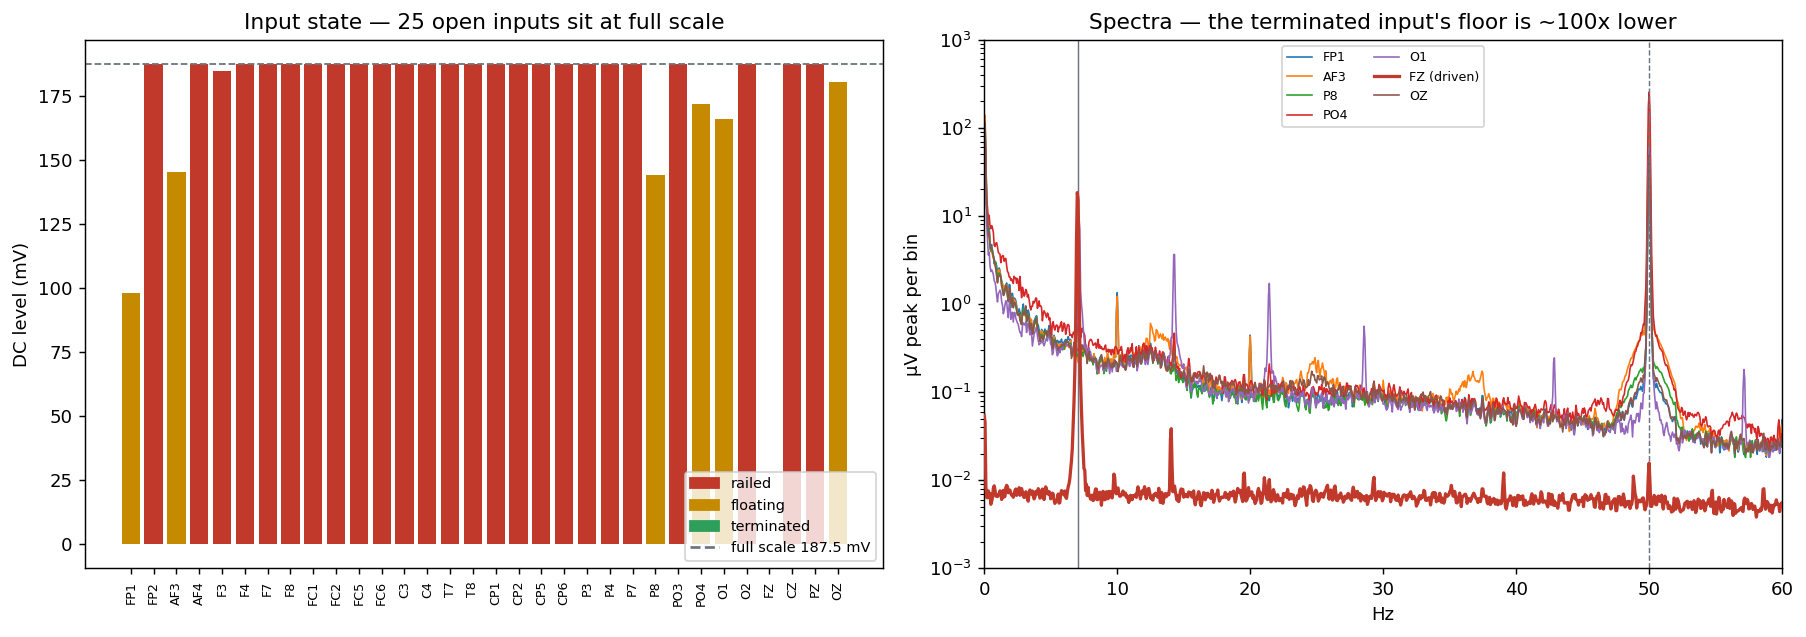
\includegraphics{../results/crosstalk7_state.png}
\caption{左:各输入的直流电平,25 个正好落在满量程。右:7 个未饱和通道的幅度谱。终接通道(红)
的本底比悬空通道低约两个数量级,且几乎没有 \SI{50}{\hertz};悬空通道带着
\SIrange{3.5}{26.5}{\micro\volt} 的工频和很大的低频漂移裙边。}
\end{figure}

\section{被驱动通道本身}

在问「漏了多少」之前,先记录唯一那个正常连接的通道表现如何 —— 这是本数据集里对放大器唯一一次
干净的表征。

\begin{table}[h]\centering\small
\caption{被驱动通道 FZ,\SI{179}{\second} 记录。}
\begin{tabular}{lrl}
\toprule
幅度 & \SI{24.542}{\micro\volt} 峰值 & \SI{17.354}{\micro\volt} 有效值 \\
幅度稳定性 & $24.05 \pm 0.03$~\uV & 连续 35 个 \SI{5}{\second} 窗口 \\
频率 & \SI{7.0226}{\hertz} & 相对标称 \SI{7}{\hertz} 偏 $+3235$\,ppm \\
THD($2f$–$6f$) & \SI{0.22}{\percent} & \\
\SI{50}{\hertz} & \SI{0.0045}{\micro\volt} & \\
本底噪声 \SIrange{20}{45}{\hertz} & \SI{0.092}{\micro\volt} rms & \\
$f_0$ 处的纯噪声天花板 & \SI{0.066}{\micro\volt} & 零分布的 95 分位 \\
\bottomrule
\end{tabular}
\end{table}

两点说明。其一,\SI{25}{\hertz} 带宽上 \SI{0.092}{\micro\volt} rms 与 ADS1299 数据手册在增益 24
下的输入折合噪声一致,说明输入正常终接时放大器是按规格工作的(详细折算见第~\ref{sec:lit} 节)。
其二,$+3235$\,ppm 的频率偏差是发生器时基与帽子采样时钟的\emph{合并}误差,单凭这段记录无法把它
归到哪一边。这个量级对晶振来说太大了($\approx$20\,ppm),所以大部分应当来自其中一个振荡器
「标称而非校准」—— 一个靠拨码设成「\SI{7}{\hertz}」的发生器是更可能的一方。无论如何,它小到
不影响 EEG 频段功率,却大到足以毁掉一次定频拟合(第~\ref{sec:traps} 节)。

\section{两个估计器陷阱}
\label{sec:traps}

\begin{figure}[h]\centering
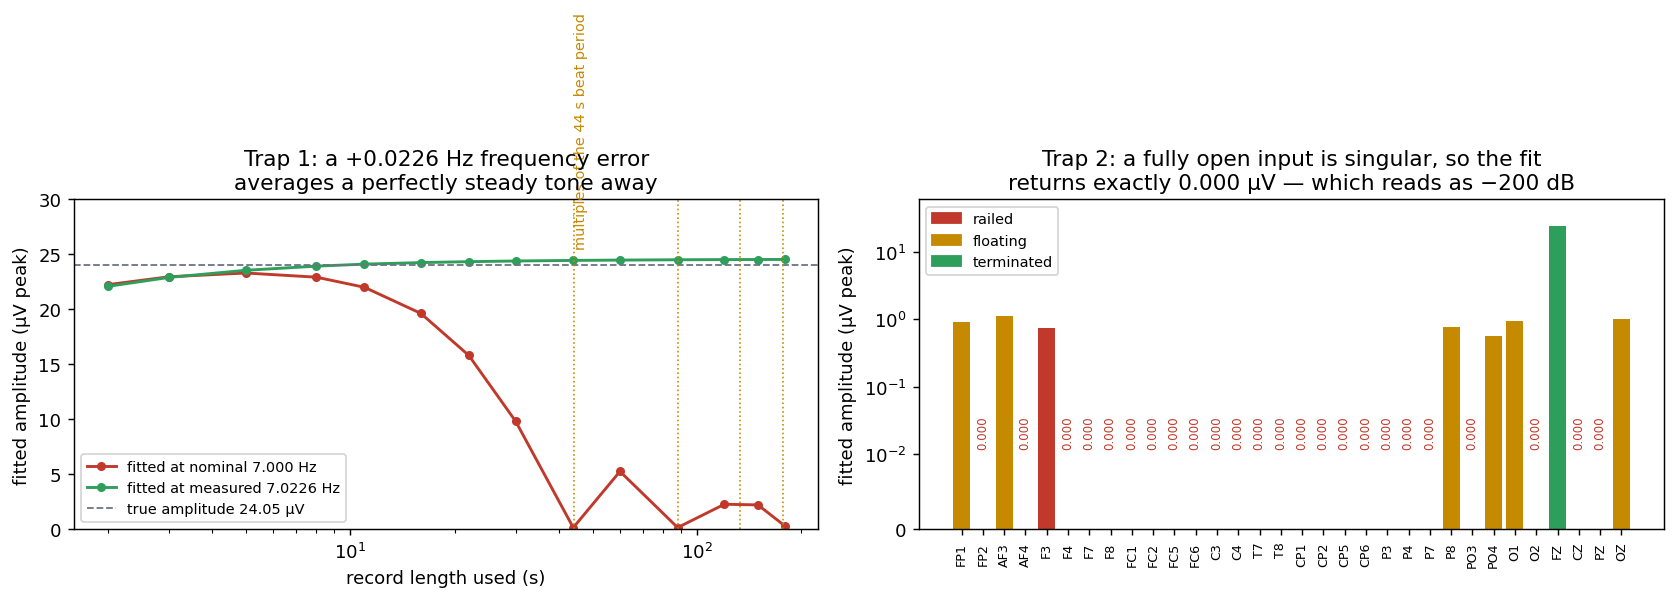
\includegraphics{../results/crosstalk7_traps.png}
\caption{左:同一个稳定的 \SI{24.05}{\micro\volt} 音调,分别在标称 \SI{7.000}{\hertz}(红)和
实测 \SI{7.0226}{\hertz}(绿)上拟合,横轴是所用记录长度。红线在 \SI{44}{\second} 拍频周期的
整数倍处塌到零。右:各通道的拟合幅度。24 个完全饱和的输入返回\textbf{正好}
\SI{0.000}{\micro\volt},因为最小二乘方程组是奇异的 —— 换算成分贝就是 $-200$,读起来像「完美
隔离」。}
\end{figure}

\paragraph{陷阱一:在标称频率上拟合。}
音调实际在 \SI{7.0226}{\hertz},不是 \SI{7.000}{\hertz}。把信号最小二乘投影到一个固定
\SI{7.000}{\hertz} 的正弦上,相位误差会以 $2\pi \times 0.0226\,t$ 累积,于是当记录跨越若干个
\SI{44}{\second} 拍频周期时,投影会把音调平均掉。在本段记录上,同一个信号读出来是:

\begin{center}\small
\begin{tabular}{lrrrr}
\toprule
所用记录长度 & \SI{11}{\second} & \SI{59}{\second} & \SI{179}{\second} & \SI{5}{\second} 分窗 \\
\midrule
在 \SI{7.000}{\hertz} 拟合 & \SI{21.84}{\micro\volt} & \SI{5.17}{\micro\volt} & \SI{0.31}{\micro\volt} & \SI{24.05}{\micro\volt} \\
在 \SI{7.0226}{\hertz} 拟合 & \SI{24.5}{\micro\volt} & \SI{24.5}{\micro\volt} & \SI{24.54}{\micro\volt} & \SI{24.05}{\micro\volt} \\
\bottomrule
\end{tabular}
\end{center}

只看第一行,信号源像是在三段连续记录里指数衰亡。它没有:全程稳定在 $\pm\SI{0.1}{\percent}$
以内。正确做法是在被驱动通道上把频率估计一次,然后所有通道都用这个频率,让源和被测方站在同一
个基准上。

\paragraph{陷阱二:饱和通道读数为零。}
对一个钉在常数上的通道,最小二乘的设计矩阵是奇异的,拟合返回\textbf{正好}
\SI{0.000}{\micro\volt}。换算成分贝是 $-200$,在结果表里和「没有串扰」完全无法区分。本次测量
的第一版里有 24 个通道落在这个状态,于是最差串扰是在剩下 6 个\emph{悬空}通道之间算出来的 ——
得到的「最差串扰 $-\SI{4.8}{\deci\bel}$」从头到尾是个伪结果。\textbf{开路通道必须报告为「无法
测量」,不能报告为零。}

\section{其它通道上到底能不能检出这个音调?}

幅度拟合永远会返回一个正数。在一个带着 \SI{1}{\micro\volt} 量级噪声裙边的漂移通道上,你要什么
频率它都会返回大约 \SI{1}{\micro\volt},所以一个绝对数值本身\textbf{什么都证明不了}。这里用的
检验把零分布建立在通道\emph{自己的噪声}上:在 \SIrange{4}{10}{\hertz} 内取 75 个频率(排除 $f_0$
及其前三次谐波)分别拟合幅度,然后问 —— 这些空频率里有多大比例返回的幅度不小于 $f_0$ 处的幅度。

\begin{table}[h]\centering\small
\caption{检出检验,\SI{179}{\second} 记录,75 个空频率。\textbf{上界}是零分布 95 分位相对
\SI{24.542}{\micro\volt} 信号源的分贝值,也就是这个通道\emph{有能力}揭示的最小泄漏。}
\begin{widetable}
\begin{tabular}{llrrrrrrl}
\toprule
通道 & 状态 & $A(f_0)$ & 零分布中位 & 零分布 p95 & $z$ & $p$ & 上界 & 判定 \\
 & & \uV & \uV & \uV & & & dB & \\
\midrule
\textbf{FZ} & 终接 & 24.542 & 0.027 & 0.066 & 1549.3 & 0.000 & $-51.3$ & \textcolor{good}{\textbf{检出音调}} \\
\midrule
O1 & 悬空 & 0.955 & 0.702 & 1.015 & 1.1 & 0.200 & $-27.7$ & 与自身噪声不可区分 \\
FP1 & 悬空 & 0.899 & 0.773 & 1.257 & 0.4 & 0.427 & $-25.8$ & 与自身噪声不可区分 \\
OZ & 悬空 & 0.995 & 0.855 & 1.382 & 0.5 & 0.427 & $-25.0$ & 与自身噪声不可区分 \\
AF3 & 悬空 & 1.131 & 0.970 & 1.522 & 0.5 & 0.440 & $-24.1$ & 与自身噪声不可区分 \\
P8 & 悬空 & 0.781 & 0.696 & 1.157 & 0.3 & 0.453 & $-26.5$ & 与自身噪声不可区分 \\
PO4 & 悬空 & 0.576 & 0.583 & 0.927 & 0.2 & 0.507 & $-28.5$ & 与自身噪声不可区分 \\
\midrule
\multicolumn{9}{l}{另有 25 个饱和通道:无法测量(在任何频率上都不携带信息)} \\
\bottomrule
\end{tabular}
\end{widetable}
\end{table}

\begin{figure}[h]\centering
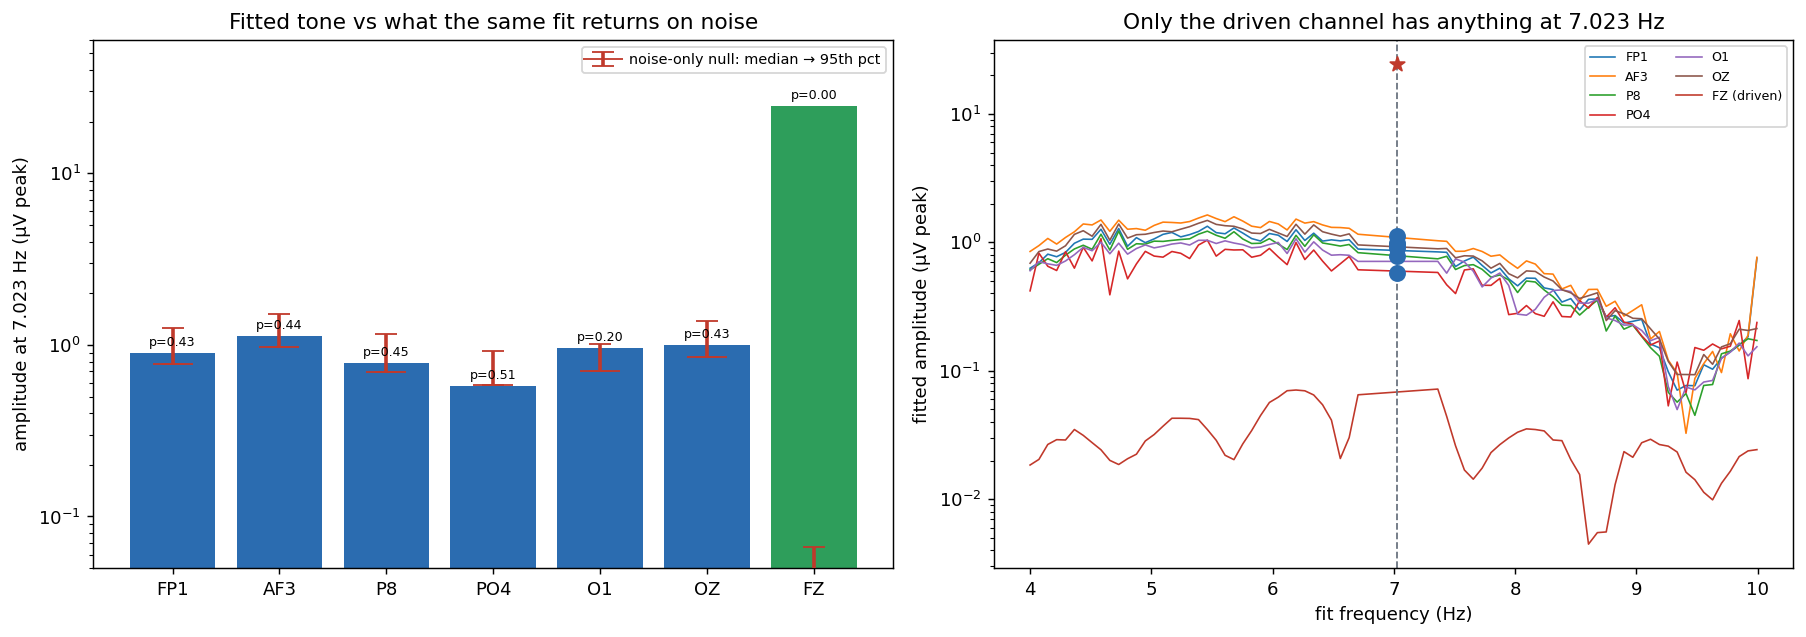
\includegraphics{../results/crosstalk7_detection.png}
\caption{左:各通道在 $f_0$ 处的拟合幅度(柱)与其纯噪声零分布的中位数和 95 分位(红)。每一个
悬空通道的「信号」都落在它自己的噪声分布之内。右:同一个拟合在频率上扫过。悬空通道画出的是一条
平滑的约 \SI{1}{\micro\volt} 曲线,\textbf{在 $f_0$ 处没有任何特征};被驱动通道在别处都是
\SIrange{0.02}{0.07}{\micro\volt},只在 \SI{7.023}{\hertz} 这一个点上冲起来。\textbf{右图一张
就是全部结论。}}
\end{figure}

\section{对照检验}

有三个量乍看像是「存在共同耦合路径」的证据。每一个都在它自己的对照下瓦解了。

\begin{figure}[h]\centering
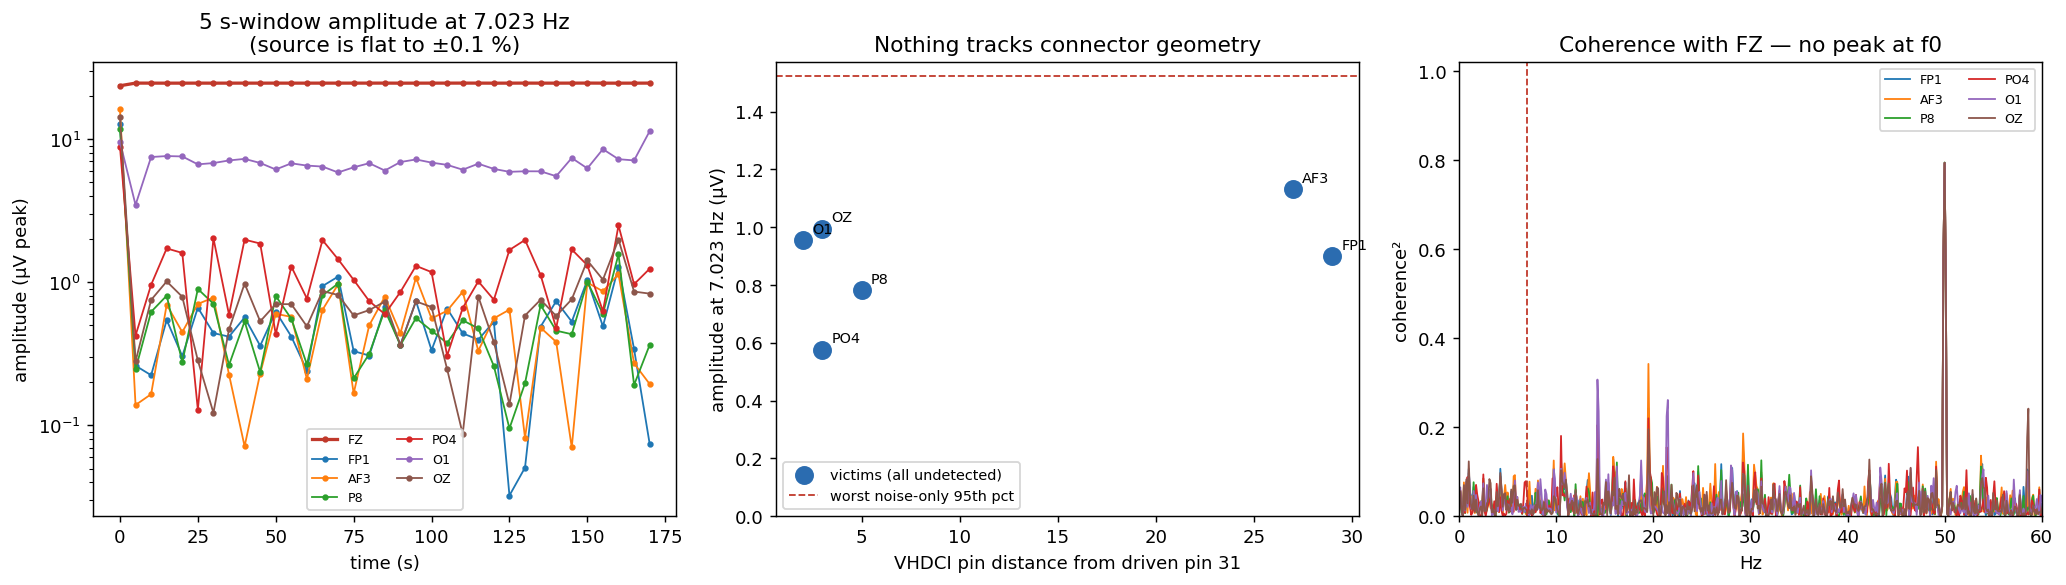
\includegraphics{../results/crosstalk7_controls.png}
\caption{左:$f_0$ 处的 \SI{5}{\second} 分窗幅度。信号源是平的,悬空通道在
\SI{1}{\micro\volt} 附近游走,与之无关。中:幅度对 VHDCI 引脚距离。右:与被驱动通道的幅度
平方相干,$f_0$ 处没有峰。}
\end{figure}

\paragraph{相位聚集。}六个悬空通道在 $f_0$ 处的相位彼此聚集在 $9.3^\circ$(圆周标准差)之内,
看起来像同一条耦合路径。但同一个统计量在 75 个空频率上的中位数是 $4.4^\circ$ —— \emph{更紧} ——
$p = 0.787$。悬空输入在几乎\textbf{每一个}频率上都彼此锁相,因为它们共享同一个环境场(两两宽带
相关中位数 $r = 0.44$)。所以 $f_0$ 处的紧聚集是零假设下就该出现的,不携带任何信息。

\paragraph{与信号源的相关。}最具决定性的对照。被驱动通道与各悬空通道的宽带 Pearson 相关系数:
$+0.0011$、$+0.0011$、$+0.0015$、$+0.0018$、$+0.0021$、$+0.0022$。\textbf{被驱动通道与帽子里
其余每一个通道都不相关。}

\paragraph{谐波。}悬空通道算出来的「THD」是 \SIrange{25}{45}{\percent},而信号源只有
\SI{0.22}{\percent}。照字面读,这说明耦合路径产生了谐波、因而是非线性的。它完全不说明这件事:
那些只是在 $14$ 和 \SI{21}{\hertz} 上对同一片宽带噪声做的拟合,而在基频本身都没被检出的前提下,
谐波比是没有意义的。

\paragraph{连接器几何。}幅度对「距被驱动的第 31 脚的引脚距离」给出 $r = +0.47$,跨度
$\Delta\text{pin} = 2$–$29$ —— 是随距离\emph{轻微上升}的,与排线导线间电容耦合应有的规律相反。
$\Delta\text{pin}=29$ 的 FP1 读数比 $\Delta\text{pin}=3$ 的 PO4 还高。这与「根本不存在几何耦合」
是一致的。

\section{复现:换一个电极,再换一个采样率}
\label{sec:repl}

一个被驱动通道只是一个数据点。把发生器移到 \textbf{FP1}(VHDCI 第 2 脚,和 FZ 的第 31 脚分处
接口两端)重测一遍,然后再用 \SI{1000}{SPS} 而非 \SI{250}{} 重测一遍。

\begin{table}[h]\centering\small
\caption{三次独立测量。\textbf{源幅度}是被驱动通道的幅度;\textbf{终接本底}是那个正常终接
通道的纯噪声 95 分位;\textbf{悬空本底}是最差悬空通道的。\textbf{上界}是悬空本底相对源幅度的
分贝值 —— 也就是这次测量\emph{有能力}揭示的最小泄漏。\textbf{最小 $p$} 是该次测量中最显著的
那个被测通道。}
\begin{widetable}
\begin{tabular}{llrrrrrrrr}
\toprule
测量 & 被驱动 & 引脚 & 源幅度 \uV & $f_0$ Hz & 终接本底 & 悬空本底 & 上界 & 最小 $p$ & $\max|r|$ \\
\midrule
FZ,\SI{250}{SPS}   & FZ  & 31 & 24.542 & 7.0226 & 0.066 & 1.522 & $-24.1$ & 0.200 & 0.002 \\
FP1,\SI{250}{SPS}  & FP1 & 2  & 24.554 & 7.0231 & 0.080 & 1.542 & $-24.0$ & 0.387 & 0.003 \\
FP1,\SI{1000}{SPS} & FP1 & 2  & 24.633 & 7.0233 & 0.065 & 1.914 & $-22.2$ & 0.400 & 0.004 \\
\bottomrule
\end{tabular}
\end{widetable}
\end{table}

\begin{figure}[h]\centering
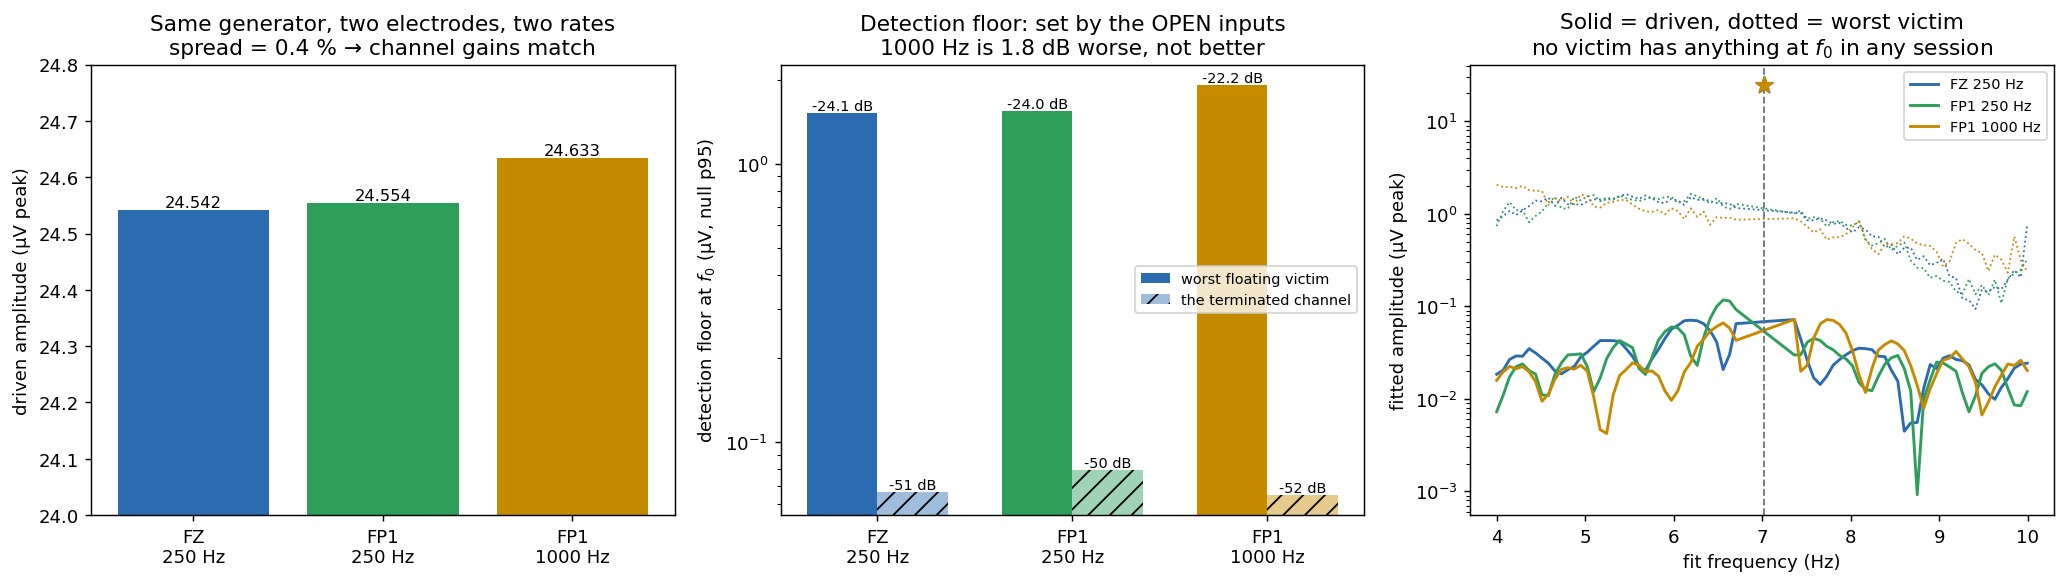
\includegraphics{../results/crosstalk7_replication.png}
\caption{左:三次测量的被驱动通道幅度,总离散 \SI{0.37}{\percent}。中:检出下限,分成终接通道
(斜纹)和最差悬空通道两部分 —— 两者之间约 \SI{27}{\deci\bel} 的差距,就是「输入不接」这件事
的全部代价。右:三次测量的扫频曲线叠在一起,实线是被驱动通道,虚线是该次最差的被测通道。
\textbf{每一条虚线都平滑地穿过 $f_0$。}}
\end{figure}

\paragraph{结论复现了。}三次测量中没有任何被测通道可检出($p = 0.20$–$0.45$),与被驱动通道的
宽带相关系数三次都低于 $0.004$,上界三次落在 \SI{2}{\deci\bel} 以内的同一个位置。驱动第 2 脚和
第 31 脚 —— VHDCI 的两端 —— 给出同样的答案,这也部分完成了第~\ref{sec:protocol} 节里「换被驱动
通道再测」那一条:无论存在什么样的导线间耦合,在接口两端都低于本底。

\paragraph{顺带得到的一个校准结果。}同一个信号源接到两个不同电极,读数是 \SI{24.542}{} 和
\SI{24.554}{\micro\volt} —— 差 \SI{0.05}{\percent};把采样率变化也算进去,三次总离散
\SI{0.37}{\percent}。数据手册给的通道间增益匹配是满量程的 \SI{0.2}{\percent}。两个通道当然算不上
一次增益普查,但就这两个而言,它们彼此吻合,也和芯片规格吻合。

\paragraph{\SI{1000}{SPS} 更差,不是更好。}这件事值得实测而不是断言,而预期成立了:上界
\emph{恶化}了 \SI{1.8}{\deci\bel},最差被测通道的噪声本底从 \SI{1.542}{} 升到
\SI{1.914}{\micro\volt}(\SI{+24}{\percent})。原因是 \SI{7}{\hertz} 处的检出下限由该处的噪声
\emph{谱密度}和总观测时长($\propto 1/\sqrt{T}$)决定,\textbf{这两样都不会因为提高采样率而改善}。
提高采样率真正改变的是:ADS1299 每个样本的内部平均变少,于是每样本输入折合噪声上升(终接通道的
\SIrange{20}{45}{\hertz} 噪声从 \SI{0.090}{} 变成 \SI{0.098}{\micro\volt} rms),同时板子要发四倍
的 UDP 流量。

对这个测量而言,\textbf{维持 \SI{250}{SPS},改成录更久}:记录时长翻倍换 \SI{3}{\deci\bel},翻四倍
换 \SI{6}{\deci\bel},代价只有时间。高采样率只有在回答另一个问题时才是对的工具 —— 耦合是否随频率
上升(这正是区分容性通路和阻性通路的特征),而那需要一个跑在几百赫兹的发生器,不是 7 Hz。

\section{这次测量确立了什么、没有确立什么}

\paragraph{确立了。}从被驱动通道漏进任何可测通道的串扰低于 \SI{-24.1}{\deci\bel}(最差通道
AF3)。放大器在输入正常终接时本底为 \SI{0.092}{\micro\volt} rms、THD \SI{0.22}{\percent}、工频
拾取可忽略。被驱动通道与其它任何通道之间未发现信号通路。

\paragraph{没有确立。}串扰究竟是 $-\SI{30}{\deci\bel}$ 还是 $-\SI{90}{\deci\bel}$。这个上界是被
\emph{被测方}的噪声卡住的,而它们中有 31 个根本没接。\SI{-24}{\deci\bel} 作为硬件指标太松了:
它允许一个通道上 \SI{50}{\micro\volt} 的 alpha 节律在邻道产生 \SI{3}{\micro\volt} —— 如果真是
这样,那是个严重缺陷。本次数据\textbf{没有任何证据说明真是这样},只是这次测量本来也看不见。

\paragraph{同样没有确立。}关于耦合\emph{机制}的任何论断。既然泄漏本身没被检出,就不存在什么
机制可以被辨识,上面那些相位、谐波和几何规律全都是噪声。

\section{要得到真正的串扰指标,该怎么测}
\label{sec:protocol}

\begin{enumerate}
\item \textbf{把所有闲置输入都接到发生器地。}这是唯一真正要紧的改动。它把被测方的本底从
约 \SI{1.0}{\micro\volt} 降到约 \SI{0.07}{\micro\volt},在同样 \SI{179}{\second}、同样信号幅度下
把上界从 $-24$ 推到约 \SI{-51}{\deci\bel}。

\item \textbf{用校准器最大的输出档。}用 \SI{2000}{\micro\volt} 代替 \SI{24.5}{\micro\volt},上界
再降 \SI{38}{\deci\bel},到约 \SI{-89}{\deci\bel} —— 已经低到与 EEG 无关。

\item \textbf{先测频率,绝不假定标称值。}在被驱动通道上调用一次 \cmd{refine()},然后所有通道都
用这个频率拟合。

\item \textbf{开路通道报告为无法测量。}绝不让一次奇异拟合变成 \SI{-200}{\deci\bel}。

\item \textbf{换被驱动通道再测一遍。}分别驱动接口一端、中间、另一端的引脚。如果哪天泄漏真的被
检出了,它对 $\Delta\text{pin}$ 的依赖关系可以区分排线导线间电容(随距离衰减)和共享的
REF/BIAS 回路(与距离无关)。

\item \textbf{发生器用电池供电},导线短且绞合。接充电器会把发生器绑到市电地,通过放大器形成
地环路。
\end{enumerate}

\section{与芯片规格、与常规实践的对照}
\label{sec:lit}

查证了两个问题:开路输入饱和是不是正常的,以及这套硬件在串扰上是否合格。

\subsection*{芯片本身就有串扰指标}

TI 的 ADS1299 数据手册(SBAS499C,表 7.5 Electrical Characteristics)给出了下列数值。它们是硅片
级典型值(增益 12、\SI{250}{SPS}),其中串扰一项正是这里要对照的。

\begin{table}[h]\centering\small
\caption{ADS1299 数据手册规格,与本次测量能看到的范围对比。}
\begin{widetable}
\begin{tabular}{llll}
\toprule
参数 & 数据手册 & 测试条件 & 本次测量 \\
\midrule
\textbf{串扰 Crosstalk} & \textbf{\SI{-110}{\deci\bel}} typ & $f_{\text{IN}} = 50/\SI{60}{\hertz}$
  & 仅上界 \SI{-24.1}{\deci\bel} \\
CMRR & \SI{-120}{\deci\bel} typ(\SI{-110}{} min) & $f_{\text{CM}} = 50/\SI{60}{\hertz}$ & 未测 \\
THD & \SI{-99}{\deci\bel} & $f_{\text{IN}} = \SI{10}{\hertz}$ & \SI{-53}{\deci\bel}(受限于发生器) \\
输入折合噪声 & \SI{1}{\micro\volt}\textsubscript{PP} typ、\SI{1.35}{} max & \SIrange{0.01}{70}{\hertz}、增益 24
  & 折算约 \SI{1.0}{\micro\volt}\textsubscript{PP} \\
输入偏置电流 & \SI{\pm 300}{\pico\ampere} & $T_A = \SI{25}{\celsius}$ & --- \\
直流输入阻抗 & \SI{1000}{\mega\ohm} & 无 lead-off & --- \\
输入电容 & \SI{20}{\pico\farad} & & --- \\
\bottomrule
\end{tabular}
\end{widetable}
\end{table}

关键对照是这一条:\textbf{芯片自己的串扰指标是 \SI{-110}{\deci\bel},而本次测量只能把串扰界定在
\SI{-24}{\deci\bel}} —— 距离「有能力检验它」还差 \SI{86}{\deci\bel}。这不是对硬件的批评,而是
对「31 个输入悬空的测量能分辨到什么程度」的陈述。板级布线和 VHDCI 排线当然可能在硅片之上再叠加
耦合,而那正是一次正确的终接测量应当去找的东西。

噪声这一项是本段记录唯一真正够到数据手册的地方。实测 \SIrange{20}{45}{\hertz}(\SI{25}{\hertz}
带宽)上 \SI{0.092}{\micro\volt} rms;按平坦谱折算到手册的 \SIrange{0.01}{70}{\hertz} 频带得
\SI{0.154}{\micro\volt} rms,再按惯用的 $6.6\sigma$ 换成峰峰值得
\SI{1.02}{\micro\volt}\textsubscript{PP},对照手册典型值 \SI{1}{\micro\volt}\textsubscript{PP}、
最大值 \SI{1.35}{}。这个外推略偏乐观 —— 真实放大器在 \SI{10}{\hertz} 以下有 $1/f$ 区,而
\SIrange{20}{45}{\hertz} 的测量看不到它,所以真实宽带值会略高于
\SI{1.02}{\micro\volt}\textsubscript{PP}。即便如此,终接通道仍落在手册的「典型到最大」区间内。
\textbf{模拟前端是称职的。}

\subsection*{开路输入饱和是预期行为,而且是有文档的预期行为}

ADS1299 数据手册的引脚表把这条指令写得很直接 —— 每一个 \cmd{INxP}\slash\cmd{INxN} 引脚下的
脚注 (2):\emph{“Connect unused analog inputs directly to AVDD.”}(未使用的模拟输入应直接接到
AVDD。)\textbf{悬空压根不是受支持的接法。}

机理就在同一批表格里。开路输入没有直流回路,\SI{\pm 300}{\pico\ampere} 的输入偏置电流除了灌进
\SI{20}{\pico\farad} 的输入电容之外无处可去:
\[
\frac{dV}{dt} = \frac{I_{\text{bias}}}{C_{\text{in}}}
 = \frac{\SI{300}{\pico\ampere}}{\SI{20}{\pico\farad}} \approx \SI{15}{\volt\per\second},
\]
毫秒量级就把节点推到电源轨。所以\textbf{25 个通道钉在满量程不是故障,而是这颗芯片对这种接线的
教科书式响应}。

这也和更广泛的社区经验一致。OpenBCI Cyton(同样基于 ADS1299)长期有大量「RAILED」报告,原因都
追溯到输入悬空或参考接触不良;那里给出的标准说法是,所有 EEG 放大器在引脚悬空时都会这样,因为
前端阻抗极高,而标准诊断手段是把通道、参考、BIAS 三者短接在一起 —— 读数应当接近零微伏。我们的
FZ 通道正处于这个状态,它读到的是 \SI{0.092}{\micro\volt} rms。

\subsection*{串扰并不是 EEG 常见的公开指标}

在决定「拿什么去对标」时值得知道:商用科研级 EEG 放大器普遍公开 CMRR,而不是通道间串扰。
Brain Products 的 actiCHamp 标称按 IEC 60601-2-26 的共模抑制 \SI{100}{\deci\bel};IEC 针对
脑电图机的标准也是围绕幅度准确度、输入动态范围、输入噪声和频率响应展开的。所以 ADS1299 的
\SI{-110}{\deci\bel} 反而比多数放大器厂商给的更具体,而且\textbf{业界并不存在一个通用的 EEG
串扰合格线}可以拿来判定这顶帽子。真正的判据来自应用本身:泄漏应远低于最小的有用信号 —— 对 MI
而言,一个通道上 \SI{50}{\micro\volt} 的节律不应在邻道产生可观的亚微伏,大致对应
\textbf{\SI{-40}{\deci\bel} 或更好}这个工作要求。

\subsection*{关于硬件质量的结论}

本次测量\textbf{没有任何迹象表明存在串扰问题},而且有一个通道的证据表明模拟前端达到了数据手册
的噪声规格。但这次测量\textbf{不足以给这顶帽子出具合格证}:\SI{-24}{\deci\bel} 的上界比
\SI{-40}{\deci\bel} 的工作要求还松,所以「没发现问题」还不等于「验证合格」。第~\ref{sec:protocol}
节的终接测量协议可以补上这个缺口,代价是一个晚上。

\section*{参考来源}

\begin{itemize}\small
\item Texas Instruments, \emph{ADS1299-x Low-Noise, 4-, 6-, 8-Channel, 24-Bit ADCs for
Biopotential Measurements}, SBAS499C, 2017 年 1 月修订 —— 第 7.5 节 Electrical Characteristics
(串扰、CMRR、THD、输入折合噪声、输入偏置电流、输入电容、直流输入阻抗)与第 6 节 Pin Functions
(“Connect unused analog inputs directly to AVDD”)。
\url{https://www.ti.com/lit/ds/symlink/ads1299.pdf}
\item OpenBCI 社区论坛,基于 ADS1299 的 Cyton 板关于悬空/参考接触不良导致 railed 的讨论串。
\url{https://openbci.com/forum/index.php?p=/discussion/3056/electrode-cap-all-channels-are-railed-resolved}
\item Brain Products GmbH, actiCHamp 系列规格(CMR \SI{100}{\deci\bel},按 IEC 60601-2-26)。
\url{https://www.brainproducts.com/solutions/actichamp/}
\item IEC 60601-2-26:2012, \emph{Medical electrical equipment --- Part 2-26: Particular
requirements for the basic safety and essential performance of electroencephalographs}.
\url{https://webstore.iec.ch/en/publication/2637}
\end{itemize}

\section*{数据与复现}

\begin{center}\small
\begin{tabular}{ll}
\toprule
\cmd{recordings/calibrator/cal\_7hz\_180s.npz} & 驱动 FZ,\SI{250}{SPS},\SI{179}{\second} \\
\cmd{recordings/calibrator/cal\_7hz\_fp1\_250sps\_180s.npz} & 驱动 FP1,\SI{250}{SPS} \\
\cmd{recordings/calibrator/cal\_7hz\_fp1\_1000sps\_180s.npz} & 驱动 FP1,\SI{1000}{SPS} \\
\cmd{recordings/calibrator/cal\_7hz\_xt7hz\_60s.npz} & FZ,\SI{59}{\second} \\
\cmd{recordings/calibrator/cal\_7hz\_probe11s.npz} & FZ,\SI{11}{\second} \\
\cmd{results/crosstalk7.json}、\cmd{xt\_fp1\_250.json}、\cmd{xt\_fp1\_1000.json} & 本报告中的每一个数字 \\
\bottomrule
\end{tabular}
\end{center}

\begin{shell}
python src/acquisition/crosstalk_analysis.py \
    recordings/calibrator/cal_7hz_180s.npz --freq 7 --json results/crosstalk7.json
\end{shell}

所有记录都是原始 \si{\micro\volt}、未滤波、未重参考,\textbf{32 导全部保留}。

\end{document}
